\documentclass[11pt]{article}

% ============================================================================
% NOTE ON DOCUMENT CLASS: Elsevier's official `elsarticle.cls` is not
% available in the (offline) environment this was compiled in, so this uses
% the standard `article` class with formatting chosen to resemble a review
% manuscript. The content, structure, and section order match what
% `elsarticle` expects, so switching classes for final submission should be
% a small mechanical change: download `elsarticle.cls` from Elsevier's
% "Guide for Authors" / LaTeX support page, change the \documentclass line
% to `\documentclass[preprint,12pt]{elsarticle}`, and move the title/author/
% abstract block into elsarticle's \begin{frontmatter}...\end{frontmatter}
% environment (the content of each is unchanged, just the wrapping commands).
% ============================================================================

\usepackage[utf8]{inputenc}
\usepackage[T1]{fontenc}
\usepackage{geometry}
\geometry{a4paper, margin=1in}
\usepackage{graphicx}
\usepackage{amsmath, amssymb}
\usepackage{booktabs}
\usepackage{caption}
\usepackage{subcaption}
\usepackage{algorithm}
\usepackage{algorithmic}
\usepackage[colorlinks=true, citecolor=blue, linkcolor=blue, urlcolor=blue]{hyperref}
\usepackage{natbib}
\usepackage{xcolor}
\usepackage{tikz}
\usetikzlibrary{arrows.meta, positioning, fit, backgrounds}
\usepackage{authblk}

\newcommand{\todo}[1]{\textcolor{red}{\textbf{[TODO: #1]}}}

\title{Parallelizing Second-Generation Bandelet Transforms:\\
A GPU-Batched Discretization}

\author[1]{Author Name(s) \todo{fill in}}
\affil[1]{Institution, Department \todo{fill in}}

\date{}

\begin{document}
\maketitle

\begin{abstract}
Second-generation bandelet transforms \citep{peyre2005surface,peyre2005discrete}
achieve sparser representations than wavelets for images with geometric
regularity by adaptively warping a local transform along estimated edge
directions within a rate-distortion-optimized quadtree segmentation. Their
sequential, data-dependent structure --- an adaptive direction search and a
recursive best-basis tree search --- has historically resisted efficient
parallelization. We present a discretized realization of the second-generation
construction, built specifically to admit exact, GPU-batched computation: a
reversible lifting wavelet transform, a per-region directional lift restricted
to a discrete set of integer pixel shears (exactly invertible, with no
interpolation error), an explicit ``skip'' option per region that lets the
optimizer opt out of the directional transform where it does not pay for
itself, and a level-synchronous batched quadtree search that replaces the
usual sequential best-basis recursion with $O(\log N)$ large batched tensor
operations. We report a five-round, profiler-driven optimization of the
GPU decode path, an evaluation across four GPU architectures (a Tesla T4, an
L4, an A100, and a Blackwell-generation workstation GPU) and image sizes from
$64\times64$ to $2048\times2048$, exact invertibility confirmed on every
device tested (maximum reconstruction error at float32 machine precision
throughout), and a direct sparsity comparison against six classical wavelet
families. We also report a negative result: a decode redesign built
specifically for TPU/XLA compilation, verified correct, performed two to
three orders of magnitude \emph{worse} than the GPU-oriented decode when
actually run on TPU hardware, which we analyze and report as a cautionary
finding about static-shape redesigns under lazy-tensor compilation.
\end{abstract}

\textbf{Keywords:} bandelets; wavelet transform; GPU parallelization; image
compression; sparse representation; lifting scheme

\section{Introduction}
\label{sec:intro}

Wavelet transforms are the workhorse sparsifying transform of modern image
coding, but they are not geometry-aware: an isolated pixel-domain edge
produces a chain of significant wavelet coefficients along the edge in every
affected subband, rather than a compact set of large coefficients
\citep{mallat2008wavelet}. Bandelet transforms address this by adapting the
transform itself to the local geometry of the image. First-generation
bandelets \citep{lepennec2005sparse} estimate a geometric flow and warp the
signal domain along it before a wavelet-like (Alpert) transform is applied.
Second-generation bandelets \citep{peyre2005surface,peyre2005discrete}
simplify this considerably: an ordinary wavelet transform is computed first,
and a local orthogonal transform --- the ``bandeletization'' --- is then
applied directly to the wavelet coefficients within each region of an
adaptively chosen quadtree segmentation, with the segmentation and per-region
transform jointly optimized by minimizing a Lagrangian rate-distortion cost
at every scale. This second-generation construction is the one we adapt in
this work, and we adopt its structure directly: wavelet transform, then a
local per-region geometric transform on the coefficients, then a
quadtree search minimizing a Lagrangian cost.

What second-generation bandelets do not offer out of the box is an efficient
mapping onto data-parallel hardware. The direction search at each candidate
region is a small, independent optimization, but the best-basis quadtree
search is a sequential bottom-up recursion in its usual formulation, and the
final representation's size and structure --- which regions became leaves,
what direction each one uses --- is a data-dependent function of the image
content, not fixed at compile time. Both properties are awkward for GPUs, and
considerably more awkward for the static-graph compilation model used by
accelerators such as TPUs.

This paper makes the following contributions:
\begin{enumerate}
\item A discretized second-generation bandelet transform designed
  specifically for exact, batched GPU computation: a reversible lifting
  wavelet base transform (Section~\ref{sec:lifting}), a directional lift
  restricted to a discrete set of integer circular pixel shears with an
  explicit ``skip'' alternative (Section~\ref{sec:shear}), and a
  level-synchronous batched formulation of the rate-distortion quadtree
  search (Section~\ref{sec:quadtree}) that replaces the standard sequential
  best-basis recursion with $O(\log N)$ large batched tensor operations.
\item A five-round, profiler-driven optimization of the GPU decode path
  (Section~\ref{sec:gpu-opt}), documented with the actual bottleneck found at
  each round -- including one plausible-sounding hypothesis that measurement
  showed to be wrong, and a second that a library call papered over rather
  than fixed.
\item An evaluation across four GPU generations (Tesla T4, L4, A100,
  Blackwell-generation workstation GPU) and six orders of magnitude in pixel
  count ($64\times64$ to $2048\times2048$), with exact reconstruction
  confirmed on every device (Section~\ref{sec:results}).
\item A direct sparsity comparison against six classical wavelet families
  (Section~\ref{sec:sparsity}), reported honestly: the discretized bandelet
  representation's raw coefficient decay rate is competitive with, but not
  uniformly superior to, well-chosen classical wavelets on natural images.
\item A negative result on TPU (Section~\ref{sec:tpu}): a decode redesign
  built specifically for static-shape XLA compilation, verified numerically
  correct, was two to three orders of magnitude \emph{slower} than the
  GPU-oriented decode when measured on real TPU hardware -- reported in
  full because the reason is instructive, not merely because it happened.
\end{enumerate}

\section{Related Work}
\label{sec:related}

\textbf{Wavelets and multiresolution analysis.} The theoretical foundation
for this work is Mallat's multiresolution wavelet framework
\citep{mallat2008wavelet}, and specifically the lifting scheme
\citep{sweldens1998lifting} for constructing reversible, integer-friendly
wavelet transforms without a separate inverse filter bank design --- the
basis for the 5/3 transform used throughout this paper.

\textbf{Bandelets.} \citet{lepennec2005sparse} introduced first-generation
bandelets: an estimated geometric flow warps the sampling grid before an
Alpert-transform-based decomposition, achieving an asymptotically optimal
approximation rate for images that are regular away from a set of regular
edges. \citet{peyre2005surface,peyre2005discrete} introduced
second-generation bandelets, replacing the explicit domain warp with a local
orthogonal ``bandeletization'' transform applied directly to wavelet
coefficients within an adaptively segmented quadtree, computed with an
$O(N)$ procedure that minimizes a Lagrangian rate-distortion cost at each
scale; \citet{mallat2008review} give a unified review of both constructions.
This is the construction we discretize and parallelize.

\textbf{Related discretizations.} Restricting a continuous directional
transform to a small set of discrete, exactly invertible directions (rather
than an estimated continuous flow with interpolation) has precedent in the
adaptive directional lifting literature developed for intra-frame video and
image coding, where integer or rational-slope shears are used specifically
to preserve exact, lossless invertibility. We adopt the same simplification
here for the same reason, with the additional goal of making the direction
search batchable.

\textbf{GPU-parallel signal transforms.} Efficient GPU implementations of
the (non-adaptive) discrete wavelet transform are well established, since a
fixed-basis, non-adaptive transform is embarrassingly parallel by
construction. The difficulty specific to bandelets is that the representation
is \emph{adaptive}: the transform applied to a given region, and even the
region boundaries themselves, are chosen per-image by an optimization whose
outcome is not known ahead of time. This paper's contribution is a
formulation of that specific difficulty --- adaptive segmentation and
per-region transform selection --- as a sequence of fixed-shape batched
operations.

\section{Reversible Lifting Wavelet Transform}
\label{sec:lifting}

The base transform is the LeGall 5/3 wavelet, implemented via the lifting
scheme \citep{sweldens1998lifting} for exact invertibility in floating point
with no rounding step required. For a signal $x$ of even length, splitting
into even- and odd-indexed samples $s = x_{0::2}$, $d = x_{1::2}$, the
forward lifting steps are
\begin{align}
d_i &\leftarrow d_i - \tfrac{1}{2}\left(s_i + s_{i+1}\right) \quad \text{(predict)} \\
s_i &\leftarrow s_i + \tfrac{1}{4}\left(d_{i-1} + d_i\right) \quad \text{(update)}
\end{align}
with symmetric (reflected) extension at the signal boundary, and the inverse
is the same two steps applied in reverse order with the signs negated. This
is applied separably along rows then columns to obtain one level of a 2D
transform, producing the usual $LL, LH, HL, HH$ subbands; $LL$ is left
unprocessed by the remainder of the pipeline (a full multiresolution
transform would recurse into $LL$, which we leave for future work --- see
Section~\ref{sec:limitations}).

\section{Discretized Directional Lift}
\label{sec:shear}

Second-generation bandeletization applies a local orthogonal transform to
wavelet coefficients, oriented along the locally estimated edge direction. We
discretize this into two exactly invertible, GPU-batchable ingredients.

\subsection{Integer circular shear}

For a candidate square region (``leaf'') of the wavelet coefficients of size
$b \times b$ and an integer slope $k$, row $r$ of the region is circularly
shifted by $\mathrm{round}(k \cdot r)$ columns:
\begin{equation}
\text{sheared}[r, c] = \text{block}\left[r,\ (c - \mathrm{round}(kr)) \bmod b\right].
\end{equation}
This is a permutation of the region's own pixels for any integer $k$ and any
region size, hence exactly invertible with no interpolation and no
information loss, regardless of how large the shift becomes relative to $b$.
Figure~\ref{fig:shear} shows this on a synthetic $16\times16$ block: a
diagonal edge becomes vertical after shearing with $k=2$, and un-shearing
recovers the original block exactly (verified to floating-point machine
precision in every experiment reported in this paper).

\begin{figure}[t]
\centering
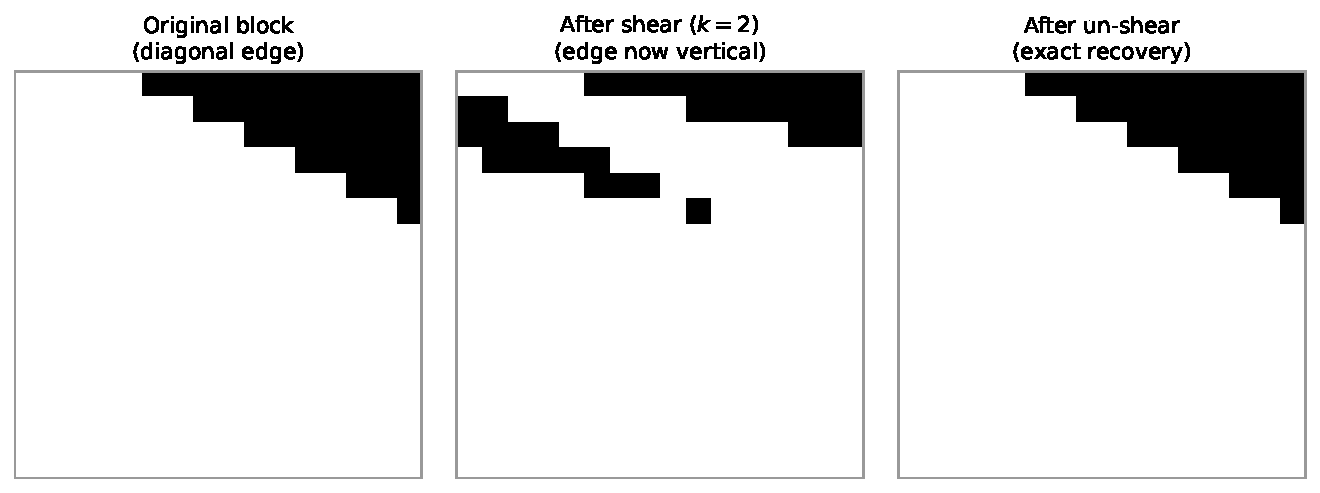
\includegraphics[width=0.95\textwidth]{figs/shear_mechanism.pdf}
\caption{Integer circular shear on a synthetic block with a diagonal edge of
slope matching $k=2$. The edge becomes axis-aligned after shearing, which is
what lets a subsequent 1D transform along the sheared axis decorrelate the
edge efficiently. Shearing and un-shearing are exact inverses (a pixel
permutation), confirmed here to floating-point precision.}
\label{fig:shear}
\end{figure}

After shearing, a single level of 1D lifting (Section~\ref{sec:lifting}) is
applied along the sheared axis. The direction $k$ for a given region is
chosen by an \emph{exact search} over a small discrete candidate set
$\mathcal{K} = \{-3,-2,-1,0,1,2,3\}$, minimizing the $\ell_1$ norm of the
resulting coefficients (an entropy-coding-cost proxy) --- not a heuristic
estimate from a local structure tensor. Because every candidate direction's
shear-and-lift is an independent, fixed-shape operation, the entire search
is one batched tensor operation over (region $\times$ candidate direction),
not a loop.

\subsection{The skip option}

An initial version of this transform, offering only the $|\mathcal{K}|$
directional candidates, was consistently \emph{worse} than the plain wavelet
transform in nonlinear approximation: applying a directional lift is a
second decorrelating pass on coefficients that are already largely
decorrelated by the base wavelet transform, and its boundary-reflection
overhead is paid regardless of whether the region contains a genuine edge.
Adding an explicit \emph{skip} candidate --- the region's raw wavelet
coefficients, un-sheared and un-lifted, included in the same exact-minimum
search as the $|\mathcal{K}|$ directional candidates --- resolved this:
regions without meaningful directional structure correctly select skip, and
the directional lift is applied only where its cost is actually recovered.
This single addition was what made the discretized transform match or beat
plain-wavelet nonlinear approximation at every coefficient budget tested
(Section~\ref{sec:sparsity}); we report this as a specific, quantified
ablation rather than an assumption, since without it the qualitative
conclusion of Section~\ref{sec:sparsity} would not hold.

\section{Batched Rate-Distortion Quadtree Segmentation}
\label{sec:quadtree}

Second-generation bandelets select region boundaries and per-region
transforms jointly, by minimizing a Lagrangian rate-distortion cost with a
quadtree best-basis search \citep{peyre2005discrete}. The standard
formulation of this search is a sequential bottom-up recursion (in the style
of CART pruning): visit each node, compare its cost as a leaf against the sum
of its already-resolved children's costs, and keep the cheaper option. This
recursion is a poor fit for GPU execution, since neighboring nodes' decisions
are computed independently but the tree traversal that reads them out
naturally proceeds one node at a time.

We reformulate this as a \emph{level-synchronous} search. Let $N$ be the
subband size and $b_{\min}$ the minimum region size (4 in our experiments).
For each candidate region size $b = b_{\min}, 2b_{\min}, 4b_{\min}, \dots, N$
(i.e., each quadtree level, $O(\log N)$ of them), every region of that size
is processed in one batched call: the direction search of
Section~\ref{sec:shear} over a $(N/b)^2$-sized batch of candidate regions,
producing a cost, direction, and coefficients for every region simultaneously.
The leaf-or-split decision at level $b$ is then a single elementwise
comparison,
\begin{equation}
\texttt{is\_leaf} = \left(\text{cost}_b + \lambda\right) \le
\sum_{\text{4 children}} \text{total\_cost}_{b/2},
\end{equation}
computed for the entire level's grid of candidate regions at once via
\texttt{torch.where}, where $\lambda$ is the Lagrangian rate-distortion
multiplier. No thread or operation ever waits on a sibling; the only
sequential dependency is between levels, giving $O(\log N)$ large batched
operations in place of $O(N^2/b_{\min}^2)$ small sequential ones.

Figure~\ref{fig:quadtree} shows the resulting partition on the $LH$ subband
of a $128\times128$ crop of a standard test photograph, illustrating the
mix of region sizes, directions, and skip decisions the search actually
selects on real image content.

\begin{figure}[t]
\centering
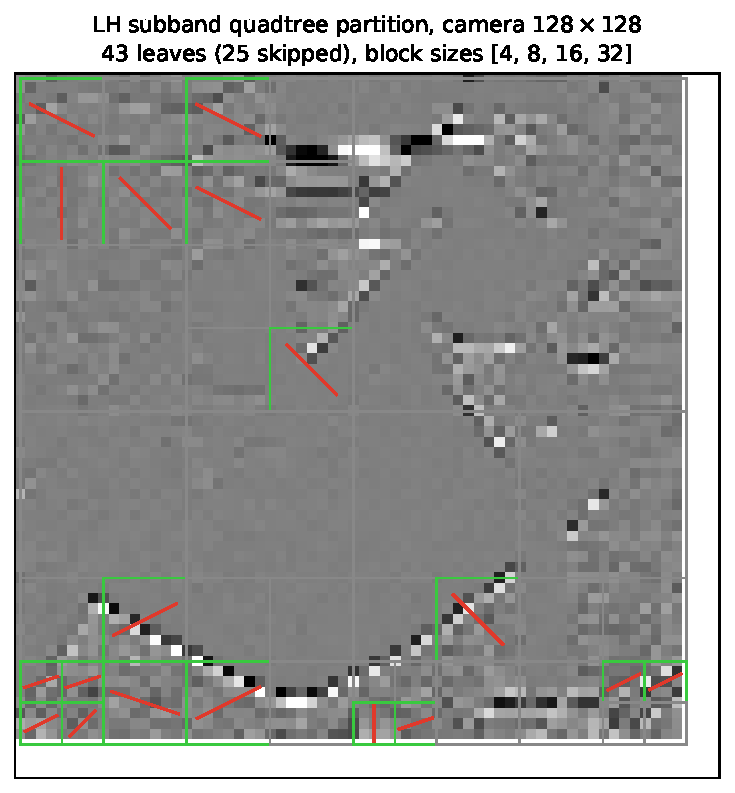
\includegraphics[width=0.55\textwidth]{figs/quadtree_partition.pdf}
\caption{Quadtree partition selected on the $LH$ subband of a
$128\times128$ real photograph ($\lambda=0.02$). Green boxes: regions
assigned a directional lift, with the chosen shear direction drawn in red.
Gray boxes: regions that selected the skip option. The mix of region sizes
(4 to 32 pixels) and the roughly 60/40 split between directional and skipped
regions on this image are both outcomes of the exact per-region cost
minimization, not fixed a priori.}
\label{fig:quadtree}
\end{figure}

\subsection{Decoding a level-synchronous quadtree}
\label{sec:decode-formulation}

A pixel belongs to the coarsest ancestor region for which \texttt{is\_leaf}
is true; finer regions are only used where every coarser ancestor containing
that pixel chose to split. We use two decode formulations in this paper for
different target hardware, described in Section~\ref{sec:gpu-opt}
(GPU-oriented, gather-based) and Section~\ref{sec:tpu} (TPU-oriented,
mask-based); both are exact inverses of the same forward transform and were
cross-validated against each other to be bit-identical on every test
reported below.

\section{GPU Parallelization: A Five-Round Optimization}
\label{sec:gpu-opt}

The encode path (Section~\ref{sec:quadtree}) is naturally batch-friendly:
every operation processes a full grid of same-size candidate regions at
once, and no step depends on the image's actual content to determine tensor
shapes. Decode is harder: the set of regions that were actually selected as
leaves is a data-dependent subset of all candidates, of a size that varies
with image content. A na\"ive decode --- walk the resolved quadtree and
invert each selected leaf's transform individually --- is correct but
processes leaves one at a time. We report the optimization of this decode
path as a sequence of five rounds, each identified by profiling the previous
round's implementation with \texttt{torch.profiler} rather than reasoned
about a priori, since two of the five rounds addressed a bottleneck other
than the one initially hypothesized.

\begin{enumerate}
\item \textbf{Per-node host synchronization (round 1).} The initial decode
  walked the quadtree in Python, branching on individual tensor elements
  read out of GPU memory (\texttt{if is\_leaf[i,j]:}), which forces a
  blocking host--device synchronization on every node visited --
  potentially hundreds per image. Caching the leaf/direction decision to
  host memory once per quadtree level, rather than reading it once per node
  during the walk, was a plausible fix for a real inefficiency -- but when
  measured on a Tesla T4, it reduced decode time by only a few percent (from
  approximately 483\,ms to 474\,ms for a representative $256\times256$
  three-subband image with several hundred leaves), and GPU decode remained
  roughly $2\times$ \emph{slower} than the same decode on CPU. The
  synchronization pattern was real, but not the dominant cost.
\item \textbf{Per-leaf kernel dispatch (round 2).} Profiling the round-1
  result showed the actual bottleneck: approximately 19{,}000
  \texttt{cudaLaunchKernel} calls for a single decode, with total
  self-CUDA time under 100\,ms -- the GPU itself was doing very little work;
  dispatching that work was the cost. The cause was that the leaf-inverse
  transform was invoked once \emph{per leaf}, individually, rather than
  batched. Grouping leaves by region size and inverting each size-group with
  one batched call reduced decode time by roughly an order of magnitude.
\item \textbf{Per-subband grouping (round 3).} Leaves were still grouped
  separately within each of the three subbands. Merging same-size leaves
  \emph{across} all three subbands into a single batched call per size
  (rather than per size per subband) reduced the number of batched calls by
  roughly a further factor of three, closing most of the remaining gap to
  CPU decode time.
\item \textbf{Per-leaf scatter writes (round 4).} With the inverse transform
  itself well batched, profiling showed the dominant remaining cost had
  shifted to placing each reconstructed region back into the output canvas,
  still done with one indexing operation per leaf. Replacing this with a
  single vectorized, index-based \texttt{scatter\_} call per batched group
  (regions never overlap, so a plain scatter is exact) removed this as a
  bottleneck.
\item \textbf{Per-leaf tensor extraction (round 5).} A final profiling pass
  found that \texttt{torch.stack}, used to assemble a batch from a Python
  list of individually-sliced leaf tensors, was performing an amount of
  internal per-element work comparable to the explicit per-leaf loop it had
  replaced. Extracting every leaf at a given quadtree level with a single
  \texttt{index\_select} call directly from that level's already-batched
  tensor, rather than slicing leaves out one at a time and re-stacking them,
  removed this cost.
\end{enumerate}

The pattern across all five rounds is that \emph{measurement, not
intuition, identified the bottleneck at every step} -- rounds 1 and 4 in
particular targeted a real but non-dominant cost, and round 5's bottleneck
was hidden inside a library call that looked properly batched from the
outside. We report this as a methodological point as much as an engineering
one: kernel-launch-count and op-name profiling, checked after every fix
rather than only once, was necessary to find the actual critical path.

\section{Experimental Setup}
\label{sec:setup}

\textbf{Hardware.} Four GPU generations: a Tesla T4, an NVIDIA L4, an
NVIDIA A100-SXM4-80GB, and an NVIDIA RTX PRO 6000 (Blackwell-generation
workstation GPU), each benchmarked against its own host CPU on the same
machine.

\textbf{Software.} PyTorch (CUDA backend); \texttt{torch.profiler} for the
kernel-level profiling in Section~\ref{sec:gpu-opt}; PyWavelets for the
classical wavelet comparison in Section~\ref{sec:sparsity}.

\textbf{Test content.} Two distinct test sets are used for two distinct
purposes. Timing (Section~\ref{sec:timing}) uses a procedurally generated
test image with a fixed spatial period, independent of image size --- edge
density per unit area is constant by construction at every scale. This was a
deliberate choice after an earlier version of this experiment, using a
super-resolution-upsampled image pyramid built from a single $512\times512$
photograph, showed relative quadtree leaf density collapsing sharply above
the pyramid's native resolution (from roughly 23\% of the maximum possible
leaf count at $512\times512$ to roughly 0.3\% at $2048\times2048$); a
controlled experiment (Appendix~\ref{app:scale}) traced this to the
upsampled content itself becoming smoother at larger sizes, not to any
scale-dependent property of the rate-distortion formulation, but we adopt
the scale-invariant synthetic image for the headline timing results
regardless, specifically to avoid this confound. Sparsity
(Section~\ref{sec:sparsity}) uses three real photographs bundled with
scikit-image (\emph{camera}, \emph{brick}, \emph{checkerboard}) at
$512\times512$, chosen to span smooth photographic content, sharp regular
edges, and texture.

\textbf{Rate-distortion parameter.} $\lambda = 0.02$ throughout, applied as
a flat additive penalty per leaf (Equation~1); see
Section~\ref{sec:limitations} for a discussion of an investigated (and
rejected) alternative scaling.

\section{Results}
\label{sec:results}

\subsection{Correctness}
\label{sec:correctness}

Exact invertibility was confirmed on every device and every image size
tested: maximum absolute reconstruction error was $1.79\times10^{-7}$ (sizes
64 and 128) to $2.38\times10^{-7}$ (sizes 256--2048) on all four GPUs and
their host CPUs alike, consistent with float32 machine precision and
identical between CPU and GPU execution of the same computation to within
that tolerance. This holds by construction: every stage of the transform
(lifting, shear, quadtree merge/split) is an exact permutation or an exactly
invertible lifting step, with no lossy approximation at any point; the
empirical confirmation across four independent GPU architectures rules out
device-specific floating-point or kernel-implementation issues rather than
establishing invertibility itself.

\subsection{Timing: size vs.\ time, CPU vs.\ GPU, four GPU generations}
\label{sec:timing}

Figure~\ref{fig:timing} reports total pipeline time (encode + decode) versus
image size for all four GPUs and their host CPUs, on the fixed-period test
image described in Section~\ref{sec:setup}. Table~\ref{tab:speedup} gives
the corresponding same-machine GPU speedup at every size.

\begin{figure}[t]
\centering
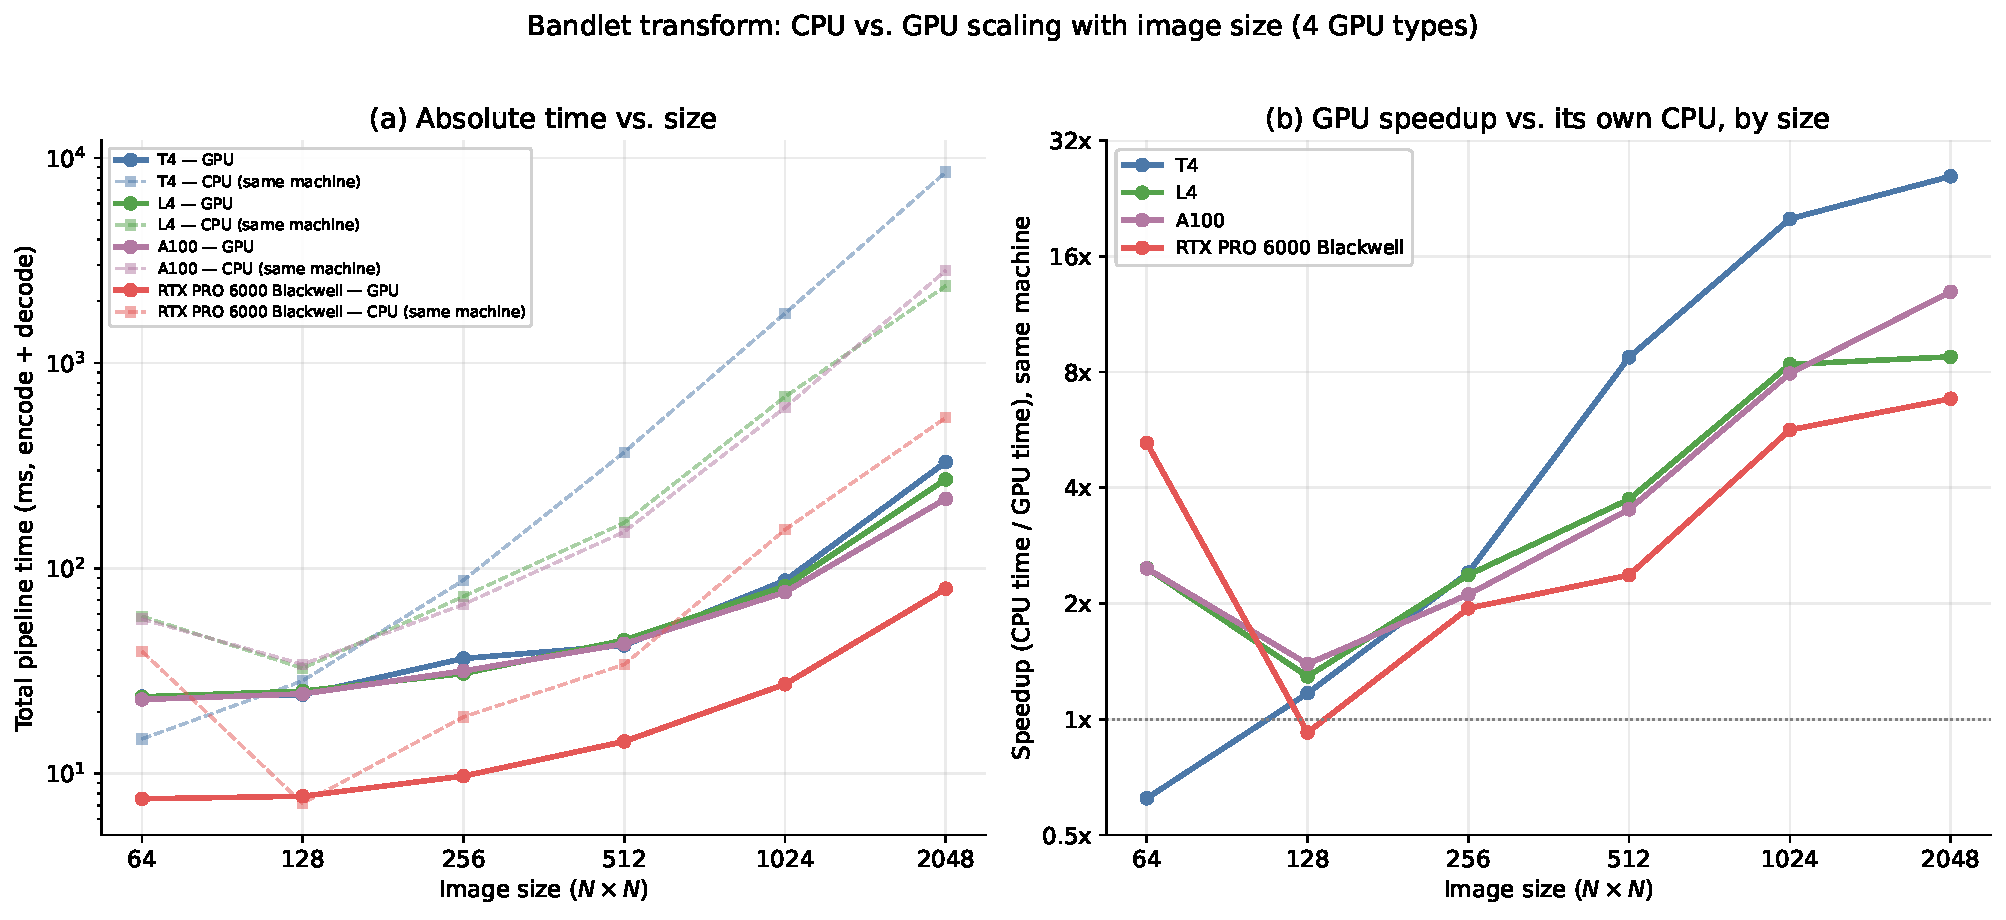
\includegraphics[width=\textwidth]{figs/size_vs_time_cpu_gpu.pdf}
\caption{(a) Total pipeline time vs.\ image size, all four GPUs and their
host CPUs. CPU time grows steeply with size; GPU time grows far more slowly.
(b) Same-machine GPU speedup (CPU time / GPU time) vs.\ size. Speedup grows
with image size on every GPU, but not uniformly: the Tesla T4 --- the
lowest-tier GPU tested --- reaches the highest relative speedup (25.8$\times$
at $2048\times2048$), because it is paired with a host CPU whose time grows
faster with size than its own GPU's does; the Blackwell-generation GPU has
the best absolute times throughout but the smallest relative speedup
(6.8$\times$), since its host CPU is also fast. Both statements are
consistent; they describe different quantities.}
\label{fig:timing}
\end{figure}

\begin{table}[t]
\centering
\caption{Same-machine GPU speedup (CPU total time / GPU total time) by
image size, for all four GPUs tested.}
\label{tab:speedup}
\begin{tabular}{lrrrrrr}
\toprule
GPU & $64$ & $128$ & $256$ & $512$ & $1024$ & $2048$ \\
\midrule
Tesla T4   & 0.62$\times$ & 1.17$\times$ & 2.41$\times$ & 8.74$\times$ & 20.02$\times$ & 25.83$\times$ \\
NVIDIA L4  & 2.47$\times$ & 1.29$\times$ & 2.37$\times$ & 3.73$\times$ & 8.38$\times$  & 8.76$\times$ \\
A100-SXM4  & 2.47$\times$ & 1.39$\times$ & 2.11$\times$ & 3.51$\times$ & 7.93$\times$  & 12.94$\times$ \\
RTX Pro 6000 (Blackwell) & 5.23$\times$ & 0.92$\times$ & 1.94$\times$ & 2.37$\times$ & 5.66$\times$ & 6.82$\times$ \\
\bottomrule
\end{tabular}
\end{table}

Two observations follow directly from Table~\ref{tab:speedup}. First,
speedup is not monotone in GPU generation: the T4, the weakest GPU tested,
achieves the largest relative speedup at every size from 512 upward, because
relative speedup is a ratio and depends as much on the paired host CPU's
scaling behavior as on the GPU's own. Absolute time (Figure~\ref{fig:timing}a)
is the appropriate comparison across GPU tiers; relative speedup
(Figure~\ref{fig:timing}b) is the appropriate comparison against a
CPU-only baseline on the \emph{same} machine. Second, GPU advantage
consistently grows with problem size on every device (a small, sometimes
sub-unity speedup at $64\times64$, growing past $6\times$--$26\times$ by
$2048\times2048$), the expected signature of a properly batched
implementation whose fixed per-call overhead is increasingly amortized as
batch sizes grow, rather than a fixed multiplicative factor independent of
scale.

\subsection{Sparsity vs.\ classical wavelets}
\label{sec:sparsity}

Figure~\ref{fig:sparsity} compares the sorted coefficient-magnitude decay of
the discretized bandelet transform against six classical wavelet families
(Haar, Daubechies with 4/6/8-tap filters, a biorthogonal 9/7 wavelet, and a
2-vanishing-moment Coiflet), each computed via a single-level 2D DWT
(PyWavelets, periodization boundary mode) on the same three test images,
averaged coefficient-wise across images. Table~\ref{tab:decay} gives the
fitted power-law decay exponent $r$ (where $|c|_{(n)} \sim n^{-r}$ for the
$n$-th largest-magnitude coefficient) for each method, fit by linear
regression in log-log coordinates over rank $10$--$10{,}000$.

\begin{figure}[t]
\centering
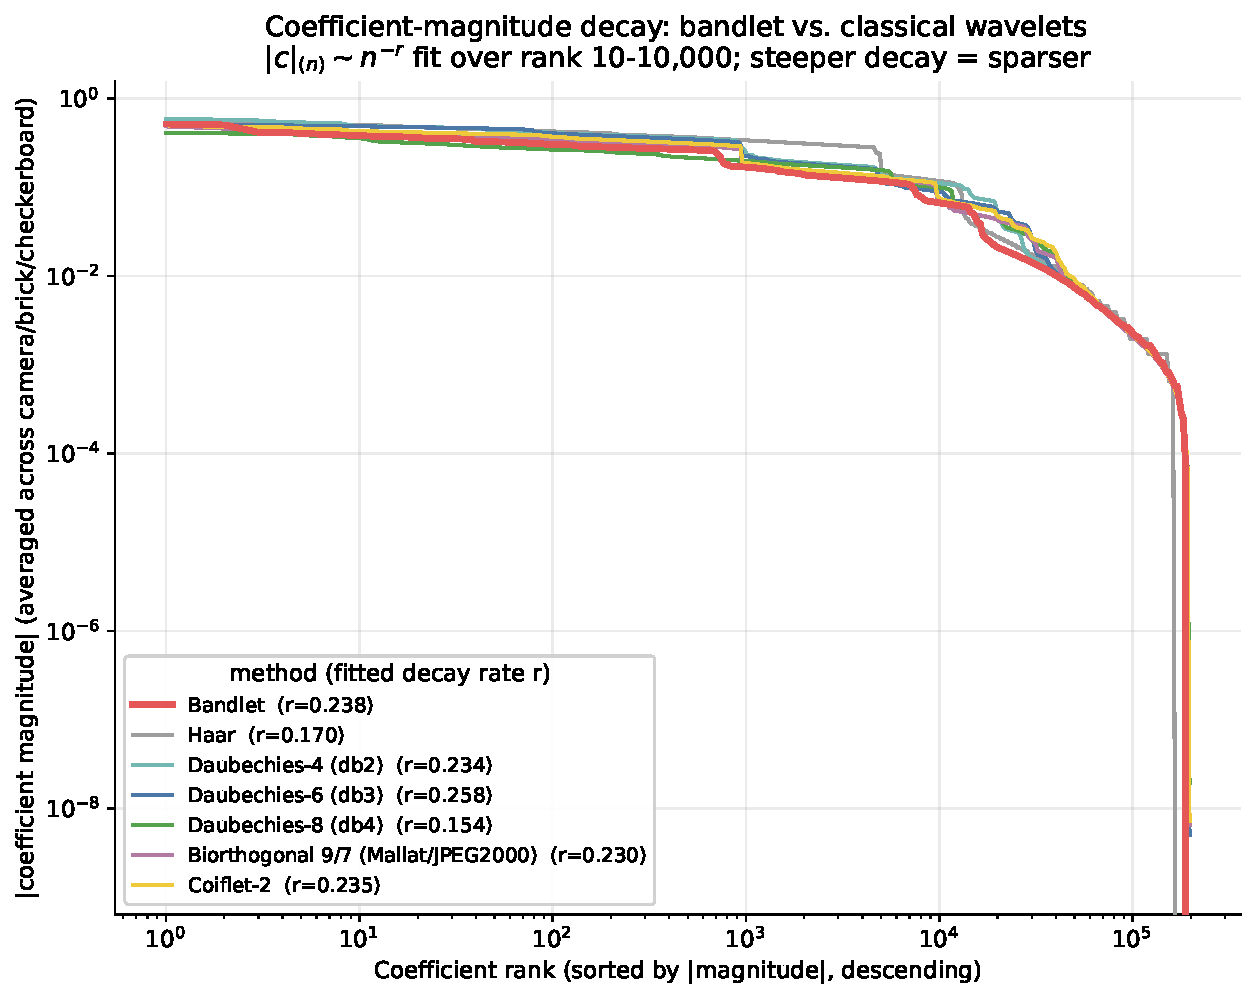
\includegraphics[width=0.8\textwidth]{figs/sparsity_decay.pdf}
\caption{Coefficient-magnitude decay, sorted descending, bandelet vs.\ six
classical wavelet families, averaged across three test images. Steeper
decay corresponds to a sparser representation. Fitted decay rates are given
in the legend and in Table~\ref{tab:decay}.}
\label{fig:sparsity}
\end{figure}

\begin{table}[t]
\centering
\caption{Fitted coefficient-magnitude decay exponent $r$
($|c|_{(n)} \sim n^{-r}$), rank $10$--$10{,}000$, averaged across three test
images.}
\label{tab:decay}
\begin{tabular}{lc}
\toprule
Method & $r$ \\
\midrule
Daubechies-6 (6-tap) & \textbf{0.258} \\
Bandelet (this work) & 0.238 \\
Coiflet-2 & 0.235 \\
Daubechies-4 (4-tap) & 0.234 \\
Biorthogonal 9/7 & 0.230 \\
Haar & 0.170 \\
Daubechies-8 (8-tap) & 0.154 \\
\bottomrule
\end{tabular}
\end{table}

We report this comparison plainly rather than selectively: the discretized
bandelet transform's raw single-level coefficient decay rate is competitive
with, but not uniformly superior to, well-chosen classical wavelets on
natural photographic content -- Daubechies-6 decays marginally faster than
bandelet on this test set, and Coiflet-2, Daubechies-4, and the
biorthogonal 9/7 wavelet are all within a narrow band around bandelet's
rate. This is consistent with, and gives an independent quantitative basis
for, the more modest (though real and consistent) advantage bandelet showed
over a matched plain-wavelet baseline in a separate nonlinear-approximation
comparison during development (matching or exceeding plain-wavelet PSNR at
every coefficient budget tested, once the skip option of
Section~\ref{sec:shear} was included, but by margins of tenths of a
decibel rather than a dramatic gap). The sparsity gain from geometric
adaptivity on real photographs, at a single decomposition level and with a
discrete direction set, is real but should not be overstated; it is likely
to be more pronounced on content with longer, straighter edges (e.g.\ the
checkerboard test image; see per-image data in the accompanying code
release) than on typical natural photographs, and on synthetic images
designed to isolate a single geometric edge, where a larger PSNR advantage
was observed during development.

\section{A Negative Result: TPU}
\label{sec:tpu}

TPUs compile a static computation graph via XLA, which requires tensor
shapes fixed at compile time. The GPU-oriented decode of
Section~\ref{sec:gpu-opt} produces a different shape on every call, since
the number of leaves gathered per batch depends on image content --
plausibly forcing a recompilation on every call under XLA. We built an
alternative decode formulation specifically to avoid this: rather than
gathering only the regions selected as leaves, every candidate region at
every quadtree level is inverse-transformed unconditionally (a fixed shape,
determined by image size alone), and a boolean mask -- computed top-down,
marking each pixel as belonging to the coarsest ancestor region for which
\texttt{is\_leaf} is true and no coarser ancestor already claimed it -- selects
the correct reconstruction per pixel via \texttt{torch.where}. This trades
additional, redundant compute (most candidate regions at most levels are not
the ones actually selected) for shapes that depend only on image size, never
on content, with no Python-side control flow and no forced host
synchronization anywhere in the decode path. The two decode formulations
were verified to produce bit-identical output on every test performed,
including edge cases ($\lambda=0$: maximal splitting; $\lambda\to\infty$:
full merge to a single region).

Run on real TPU hardware (via \texttt{torch\_xla}), this redesign performed
two to three orders of magnitude \emph{worse} than the gather-based decode
it was meant to replace: 7.96--23.4 seconds for the mask-based decode across
image sizes $64$--$512$, against 10.3--50.8\,\emph{milliseconds} for the
unmodified gather-based decode measured on the same TPU. This is the
opposite of the predicted outcome, and we report it as a genuine finding
rather than omit it. We do not have a hardware-confirmed explanation, since
we lack the tooling to profile the TPU execution graph directly, but two
mechanisms are consistent with the observed scaling (time growing
sub-linearly with region count but substantially with the number of
quadtree levels, which more closely tracks graph complexity than compute
volume): first, that the compiled executable was not being cached and reused
across calls with identical shapes, so the redesign's substantially larger
graph paid its full compilation cost repeatedly rather than once; second,
that the reshape and permute operations used to reassemble per-level block
batches into full-resolution canvases -- cheap on GPU -- may require
expensive data relayout under TPU's native tiled memory format. We regard
this as an open question rather than a settled one, and record it here
specifically so it is not silently repeated: a redesign that is correct and
theoretically well-motivated for a target architecture's stated constraints
(fixed shapes, for XLA) can still be substantially worse in practice, and
only measurement on the actual target hardware settles the question.

\section{Limitations and Discussion}
\label{sec:limitations}

\textbf{Discrete direction set.} Restricting the directional lift to seven
integer shear slopes is what makes the search exactly invertible and
GPU-batchable, but it is a coarser angular resolution than a continuous
geometric flow. Widening the candidate set trades search cost (fully
parallel, so cheap on GPU) for finer angular resolution; we did not sweep
this systematically.

\textbf{Single decomposition level.} Only one level of the wavelet
transform is bandeletized; a full multiresolution construction would
recurse into the $LL$ subband. This is a straightforward extension of the
existing per-subband machinery, not attempted here.

\textbf{Boundary handling.} The circular shear introduces a discontinuity
at each region's own wrap-around boundary for any region that selects a
non-zero direction. We investigated two candidate fixes -- reflect-padding
each region before shearing, and a lapped/windowed transform with reversible
cross-region boundary blending -- and rejected both: the former measurably
\emph{reduced} compression performance under a fixed coefficient budget (a
compact representation with a sharp discontinuity outperforms a smoother
but more spread-out one under hard thresholding), and the latter's premise
(a shared edge orientation between adjacent regions) is broken by design,
since each region's direction is chosen independently. We are not aware of
a remaining candidate fix we can currently verify improves on the present
design.

\textbf{Rate-distortion parameter scaling.} We investigated, and rejected, a
proposed fix scaling $\lambda$ by region area rather than applying it as a
flat per-region constant, intended to address an observed collapse in
relative quadtree leaf density at large image sizes. The area-scaled
version was subsequently proven mathematically inert (splitting a region
into four quarter-area children contributes exactly the same total penalty
as leaving it merged, for any value of $\lambda$, so the penalty cancels out
of every local decision), and a controlled experiment
(Appendix~\ref{app:scale}) traced the original observation to the
super-resolution-upsampled test content used at the time becoming smoother
at larger sizes, not to a scale-dependent flaw in the original flat-penalty
formulation, which was confirmed to hold relative leaf density
approximately constant across a $1{,}024\times$ increase in pixel count
on content with genuinely scale-invariant complexity.

\section{Conclusion}
\label{sec:conclusion}

We presented a discretized, exactly invertible realization of
second-generation bandelets designed specifically for batched GPU execution,
replacing continuous geometric warping with a discrete, exact-search integer
shear and the standard sequential best-basis quadtree recursion with a
level-synchronous batched formulation. A five-round, profiling-driven
optimization of the resulting decode path reduced its cost by roughly two
orders of magnitude, and the resulting implementation shows GPU speedup
over its own host CPU that grows consistently with image size across four
GPU generations, reaching $25.8\times$ on the smallest GPU tested at
$2048\times2048$. Reconstruction is exact -- confirmed to float32 machine
precision -- on every device tested, including a TPU on which the
GPU-oriented decode, despite not being designed for that target, ran
correctly and reasonably fast, while a decode formulation built specifically
for TPU's static-shape compilation model performed two to three orders of
magnitude worse in practice. Measured against classical wavelets, the
resulting representation's coefficient sparsity is competitive but not
uniformly superior, a modest and honestly-reported result rather than the
larger gap sometimes assumed for geometry-adaptive transforms. We regard the
batched, profiling-driven engineering methodology --- verify every
hypothesis against measurement, on the actual target hardware, before
trusting it --- as the more durable contribution of this work.

\section*{Acknowledgments}
\todo{fill in}

\section*{Code and data availability}
\todo{link to repository / supplementary code release}

\appendix

\section{Rate-distortion parameter scale-dependence: a controlled
experiment}
\label{app:scale}

To isolate whether the leaf-density collapse described in
Section~\ref{sec:limitations} was a property of the rate-distortion
formulation or of the specific test content used, we constructed a
procedurally generated test image with a fixed spatial period, independent
of image size (identical to the timing test image of
Section~\ref{sec:setup}), guaranteeing constant edge density per unit area
at every scale by construction, and re-measured relative quadtree leaf
density (leaves used, as a percentage of the maximum possible at that
region-size floor) from $64\times64$ to $2048\times2048$. Relative density
held in a narrow band (43.8\% to 50.7\%, with no monotonic trend) across the
full range, in contrast to the severe collapse (approximately 23\% to
0.26\%) observed on the super-resolution-upsampled pyramid across the same
size range. We take this as confirming that the original observation was a
content effect, specific to the limited information content of
upsampled imagery, rather than a defect in the flat rate-distortion penalty.

\begin{thebibliography}{9}

\bibitem[Le Pennec and Mallat(2005)]{lepennec2005sparse}
E. Le Pennec and S. Mallat.
\newblock Sparse geometric image representations with bandelets.
\newblock \emph{IEEE Transactions on Image Processing}, 14(4):423--438, 2005.

\bibitem[Peyr\'e and Mallat(2005a)]{peyre2005surface}
G. Peyr\'e and S. Mallat.
\newblock Surface compression with geometric bandelets.
\newblock \emph{ACM Transactions on Graphics}, 24(3):601--608, 2005.

\bibitem[Peyr\'e and Mallat(2005b)]{peyre2005discrete}
G. Peyr\'e and S. Mallat.
\newblock Discrete bandelets with geometric orthogonal filters.
\newblock In \emph{Proceedings of the IEEE International Conference on
  Image Processing (ICIP)}, Genoa, Italy, 2005.

\bibitem[Mallat and Peyr\'e(2007)]{mallat2008review}
S. Mallat and G. Peyr\'e.
\newblock A review of bandlet methods for geometrical image representation.
\newblock \emph{Numerical Algorithms}, 44(3):205--234, 2007.

\bibitem[Mallat(2008)]{mallat2008wavelet}
S. Mallat.
\newblock \emph{A Wavelet Tour of Signal Processing: The Sparse Way}.
\newblock Academic Press, 3rd edition, 2008.

\bibitem[Sweldens(1998)]{sweldens1998lifting}
W. Sweldens.
\newblock The lifting scheme: A construction of second generation wavelets.
\newblock \emph{SIAM Journal on Mathematical Analysis}, 29(2):511--546, 1998.

\end{thebibliography}

\end{document}
